\def\difficulty{1}
\sujet{Alpha Shapes}
\label{tut:alphashapes:enonce}

\begin{note}
The objective of this tutorial is to compute the alpha-shape of a set of points. Some tests will be done to reconstruct a shape from its random discretization as a point pattern (see Figure 1).
\end{note}


\begin{figure}[htbp]
\centering
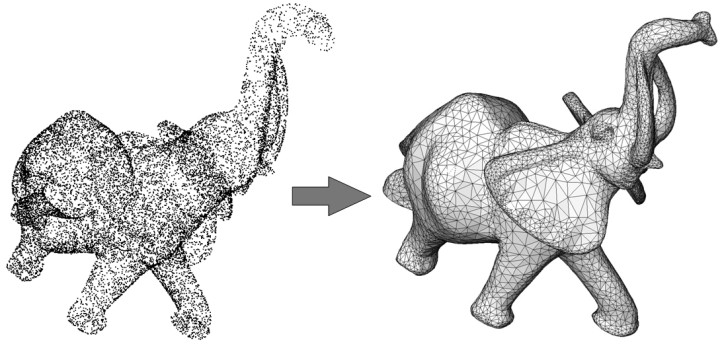
\includegraphics[width=10cm]{elephant.png}
 \caption{Shape reconstruction from a set of points.}
 \label{fig:alphashapes:elephant}
\end{figure}


\section{Point pattern}

From a binary image representing a shape, we need to extract a random set of points (included in the shape). It will define our input data.
\begin{figure}[htbp]
\centering
\subfloat[shape]{{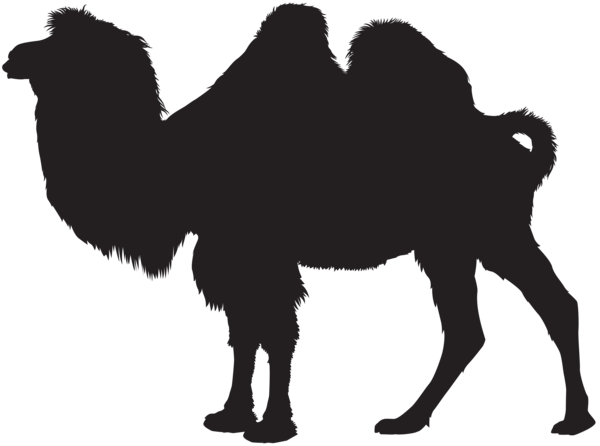
\includegraphics[width=4cm]{camel.png}}}\hspace{.5cm}
\subfloat[point pattern representing the shape]{{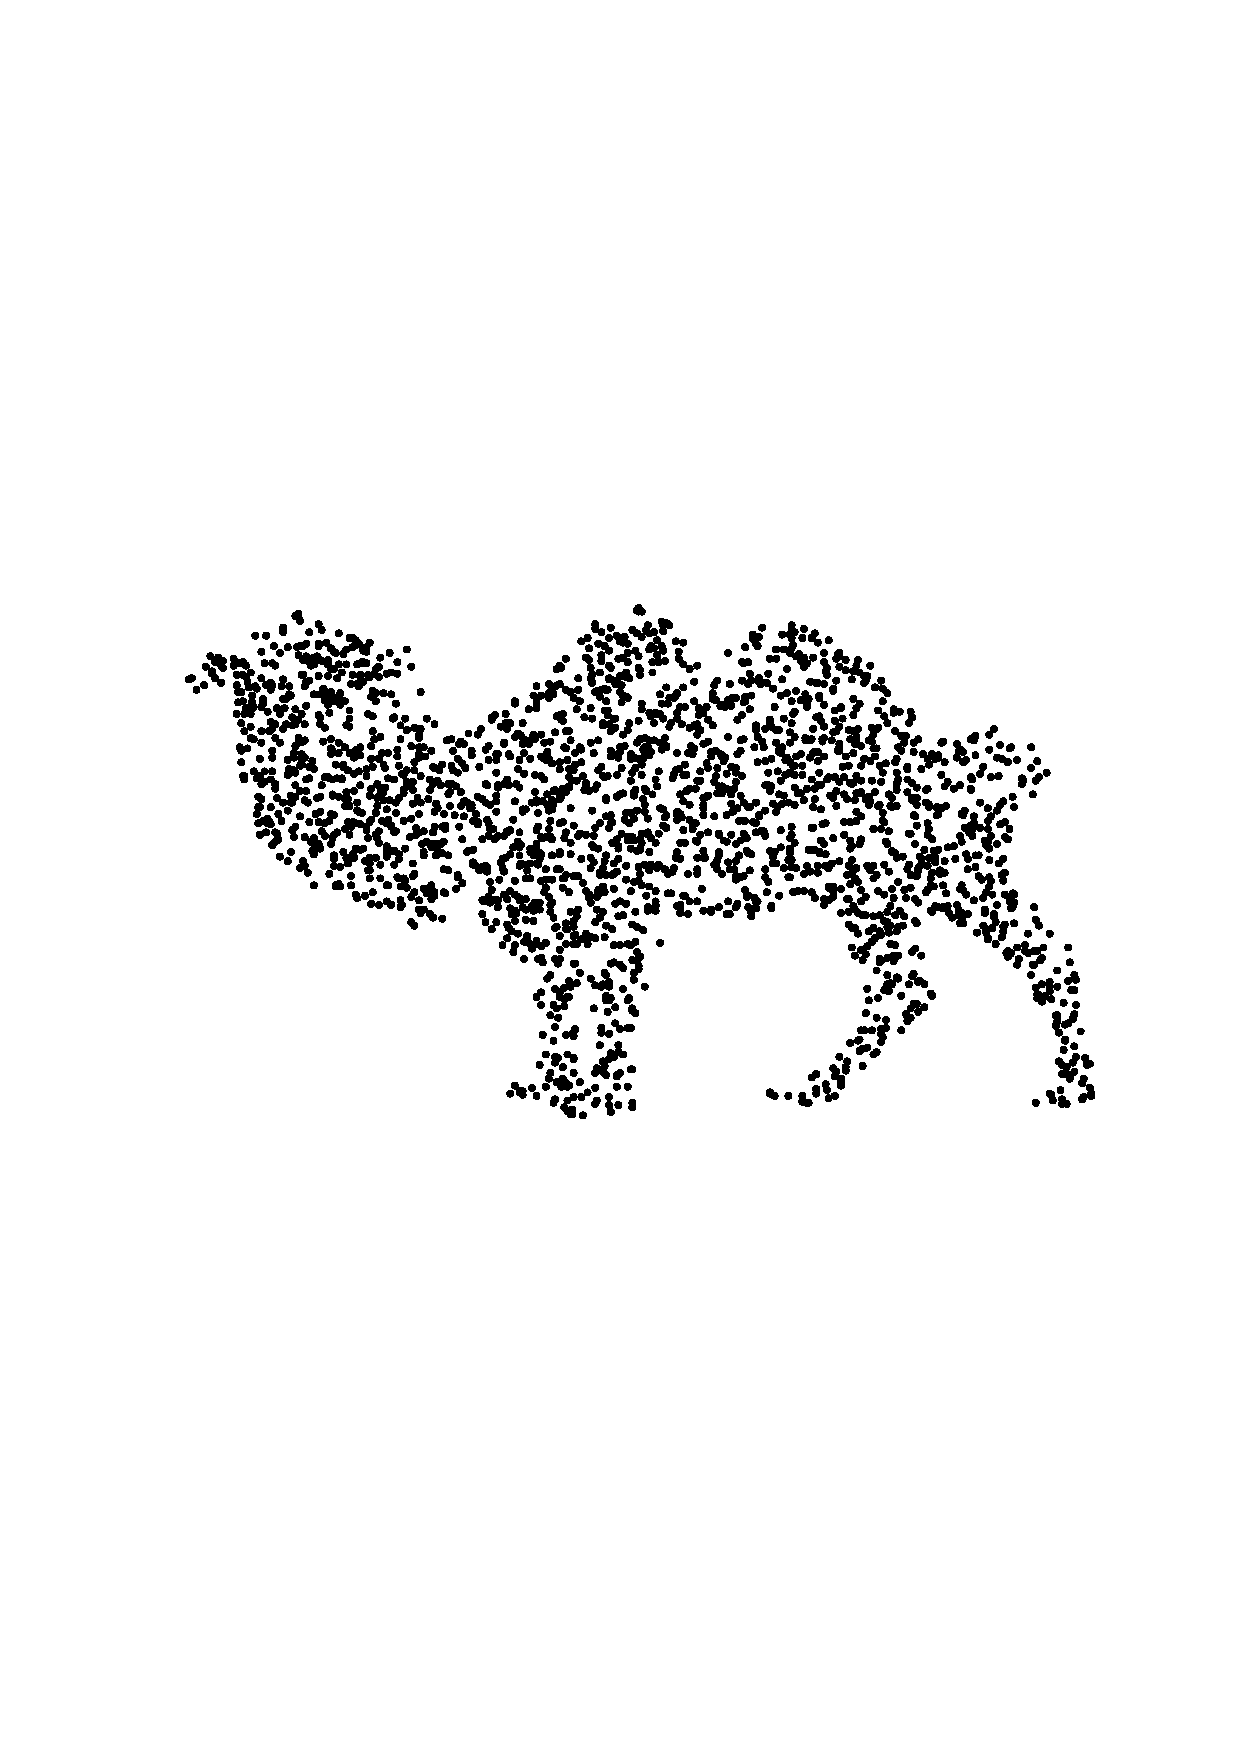
\includegraphics[width=4.25cm,height=3.75cm,trim={2.5cm 11cm 2.5cm 8cm},clip]{camel_alphashape_0.pdf}}}\hspace{.5cm}
%\subfloat[$rec(I_1,M)$]{{\includegraphics[width=3cm]{rec.jpg}}}
\caption{Shape and random discretization as a point pattern.}
\label{fig:alphashapes:pp}
\end{figure}

\begin{qbox}
\begin{enumerate}
	\item Load the image 'camel.png'.
	\item Discretize the set by using a random (uniform) point process to obtain the initial data. The density of the point process should be a user parameter.
\end{enumerate}
\end{qbox}

\begin{pcomment}
A simple way to do this is to select all discrete points that are part of the image with \pinline{np.where} and randomly select a small quantity of these points.

\begin{python}
A = imread('camel.png')
pts = np.where(A)
pts = np.array(pts).transpose()

rng = np.random.default_rng()
pts = rng.permutation(pts)

points = pts[:num_points]
\end{python}

\end{pcomment}


\section{Delaunay triangulation}

In order to build the alpha shape of a set of points, it is firstly required to compute its Delaunay triangulation.
\begin{figure}[htbp]
\centering
\subfloat[initial point pattern]{{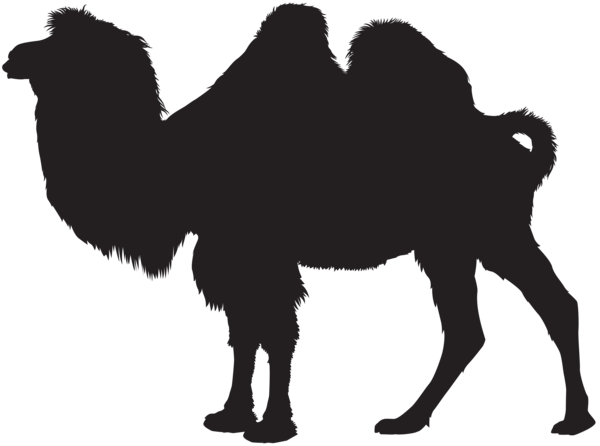
\includegraphics[width=4cm]{camel.png}}}\hspace{.5cm}
\subfloat[Delaunay triangulation]{{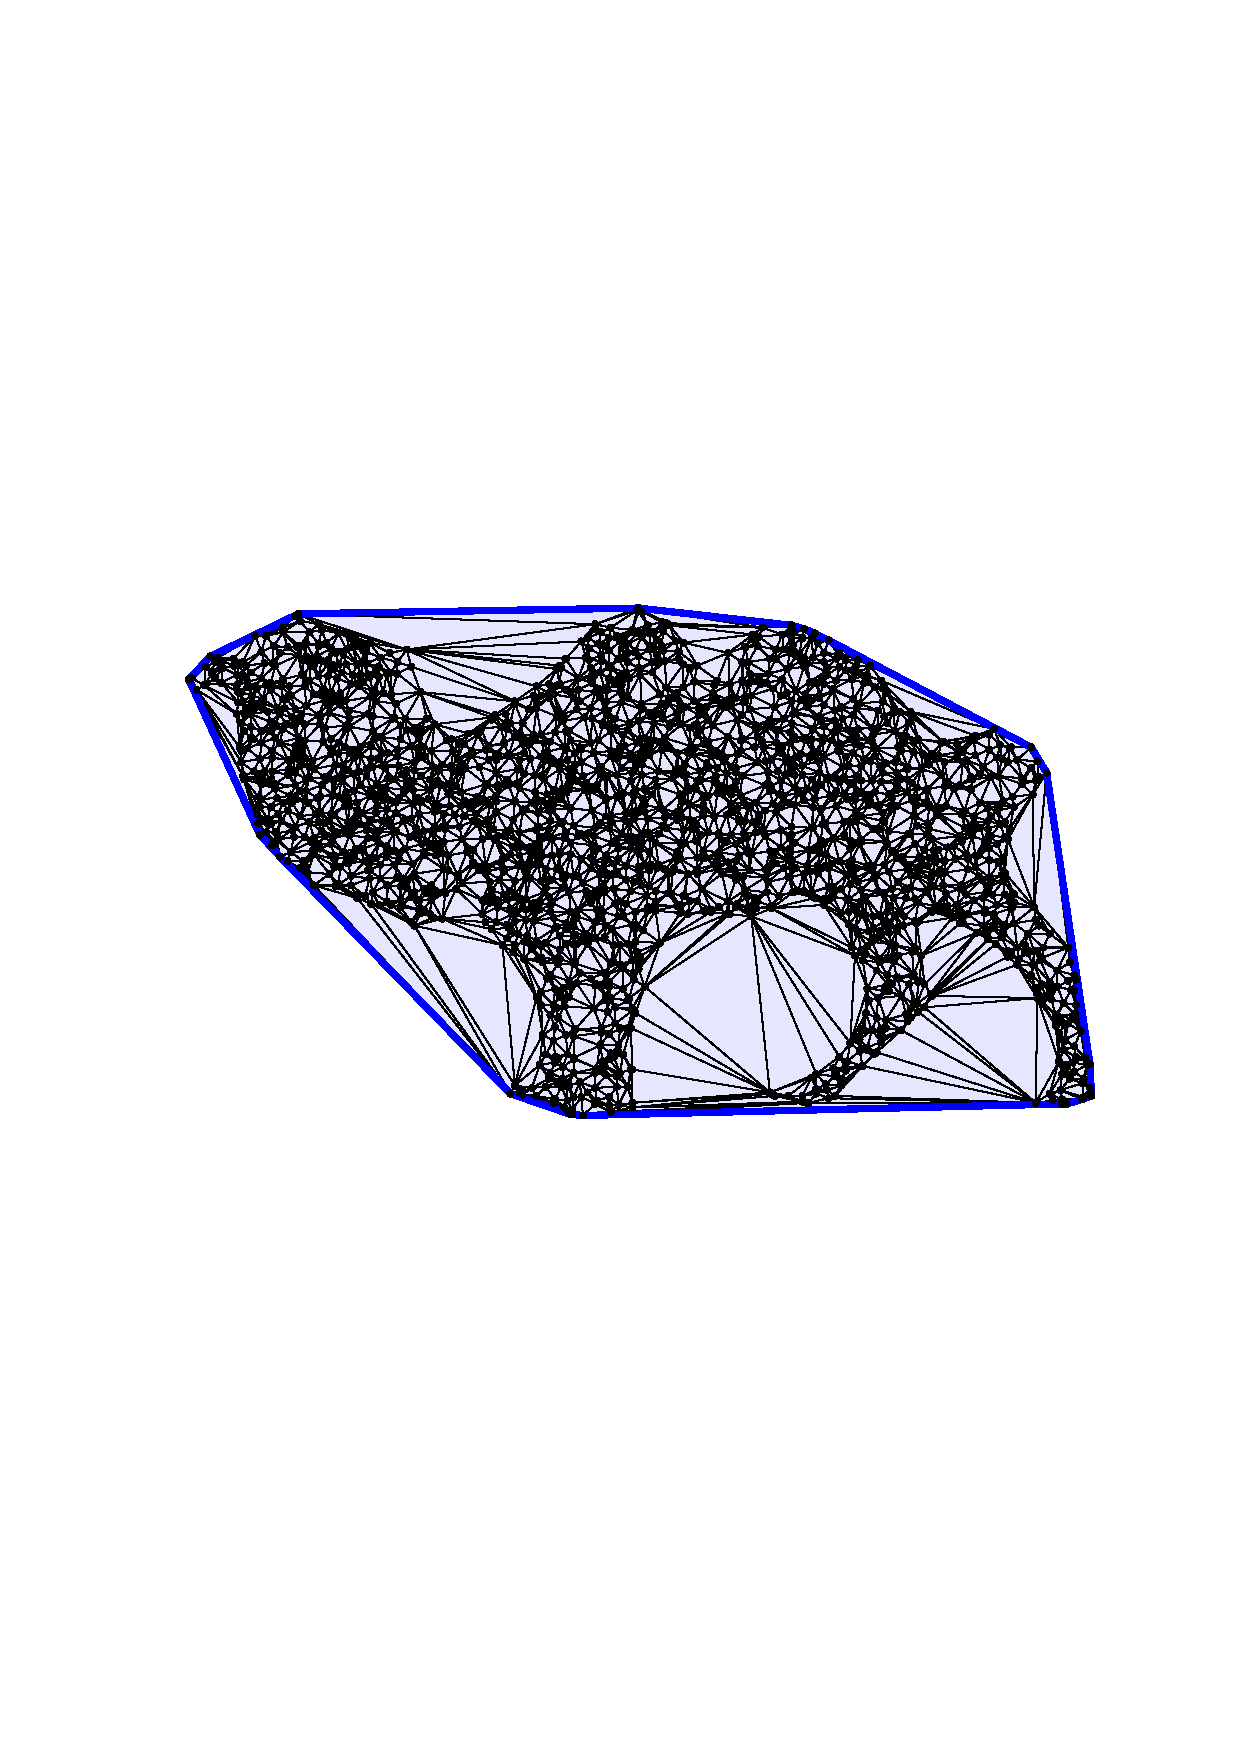
\includegraphics[width=4.25cm,height=3.75cm,trim={2.5cm 11cm 2.5cm 8cm},clip]{camel_alphashape_10.pdf}}}\hspace{.5cm}
%\subfloat[$rec(I_1,M)$]{{\includegraphics[width=3cm]{rec.jpg}}}
\caption{Initial point pattern and its Delaunay triangulation.}
\label{fig:alphashapes:delaunay}
\end{figure}

\begin{qbox}
\begin{enumerate}
	\item By using the initial point pattern, build its Delaunay triangulation.
	\item Look at the resulting object to understand the structure of the triangulation.
\end{enumerate}
\end{qbox}

\begin{mcomment}
\begin{mremark}
You can use the matlab function  \minline{delaunayTriangulation}.
\end{mremark}
\end{mcomment}

\begin{pcomment}
You can import the module Delaunay with \pinline{from scipy.spatial import Delaunay}.
 
 The display of the triangulation can be done by:
 \begin{python}
tri = Delaunay(points)
plt.triplot(points[:,0], points[:,1], tri.simplices, lw=.5)
 \end{python}


\end{pcomment}


\section{Alpha-shape}
The alpha-shape corresponds to the union of Delaunay triangles $T_{ijk}$ such that the circumradius $C_{ijk}$ is lower than $1/\alpha$.

\begin{figure}[htbp]
\centering
\subfloat[$\alpha=0.01$]{{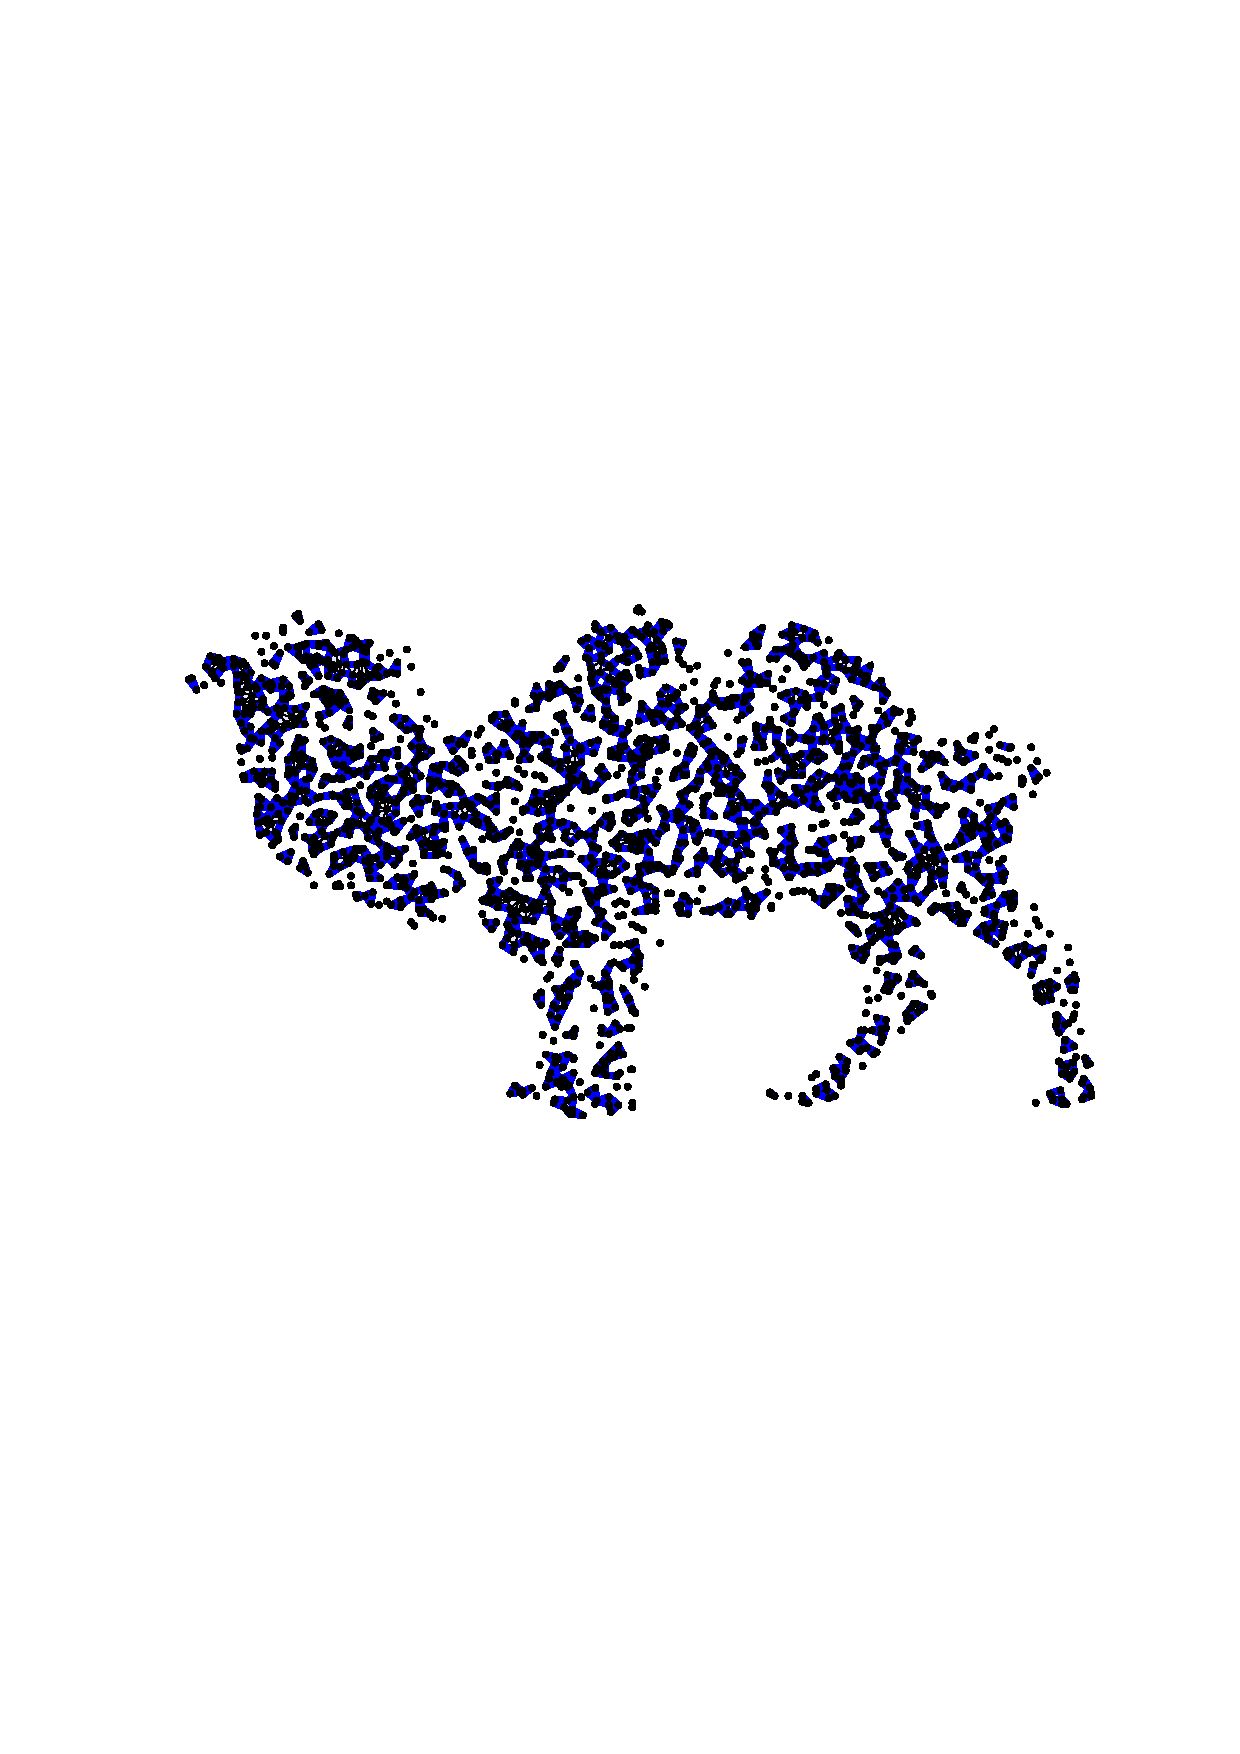
\includegraphics[width=4.25cm,height=3.75cm,trim={2.5cm 11cm 2.5cm 8cm},clip]{camel_alphashape_0.01.pdf}}}\hspace{.5cm}
\subfloat[$\alpha=0.03$]{{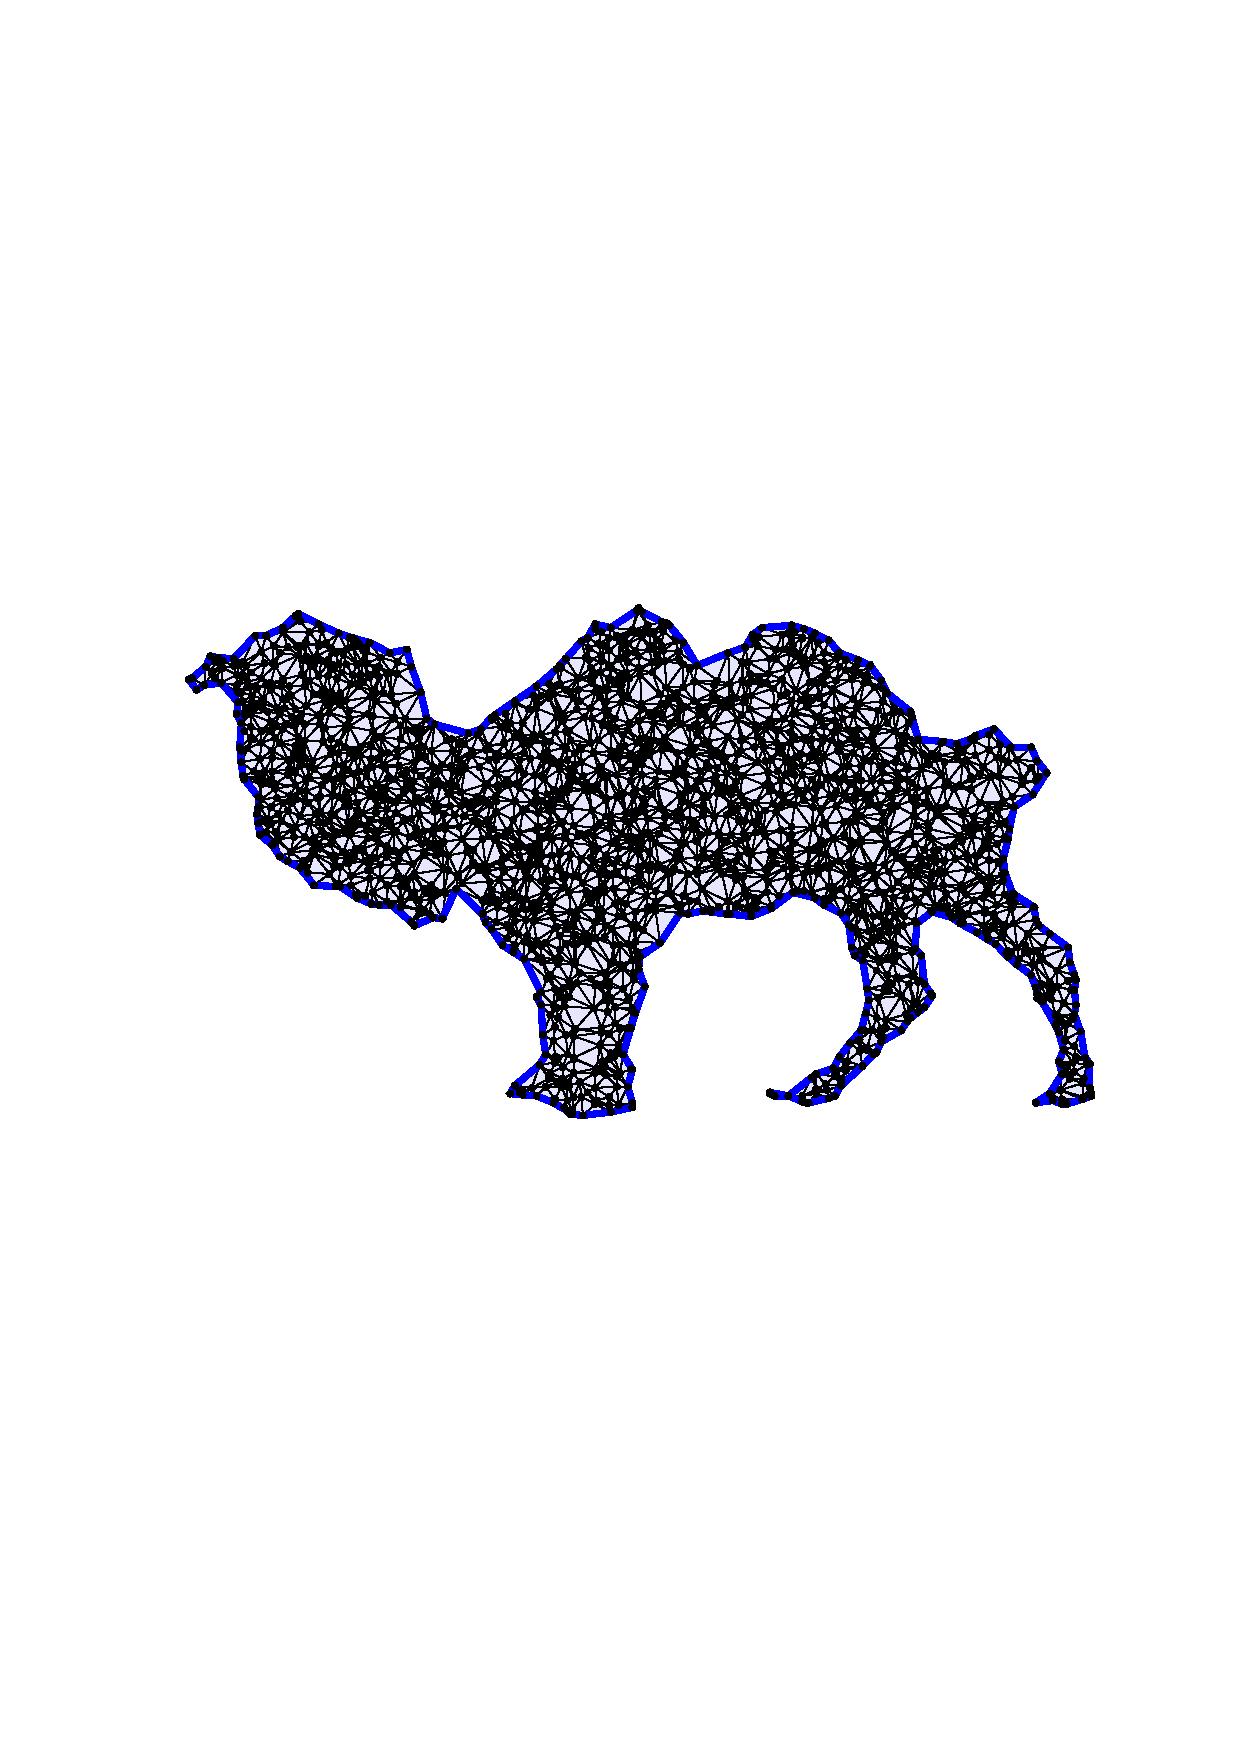
\includegraphics[width=4.25cm,height=3.75cm,trim={2.5cm 11cm 2.5cm 8cm},clip]{camel_alphashape_0.03.pdf}}}\hspace{.5cm}
\subfloat[$\alpha=0.09$]{{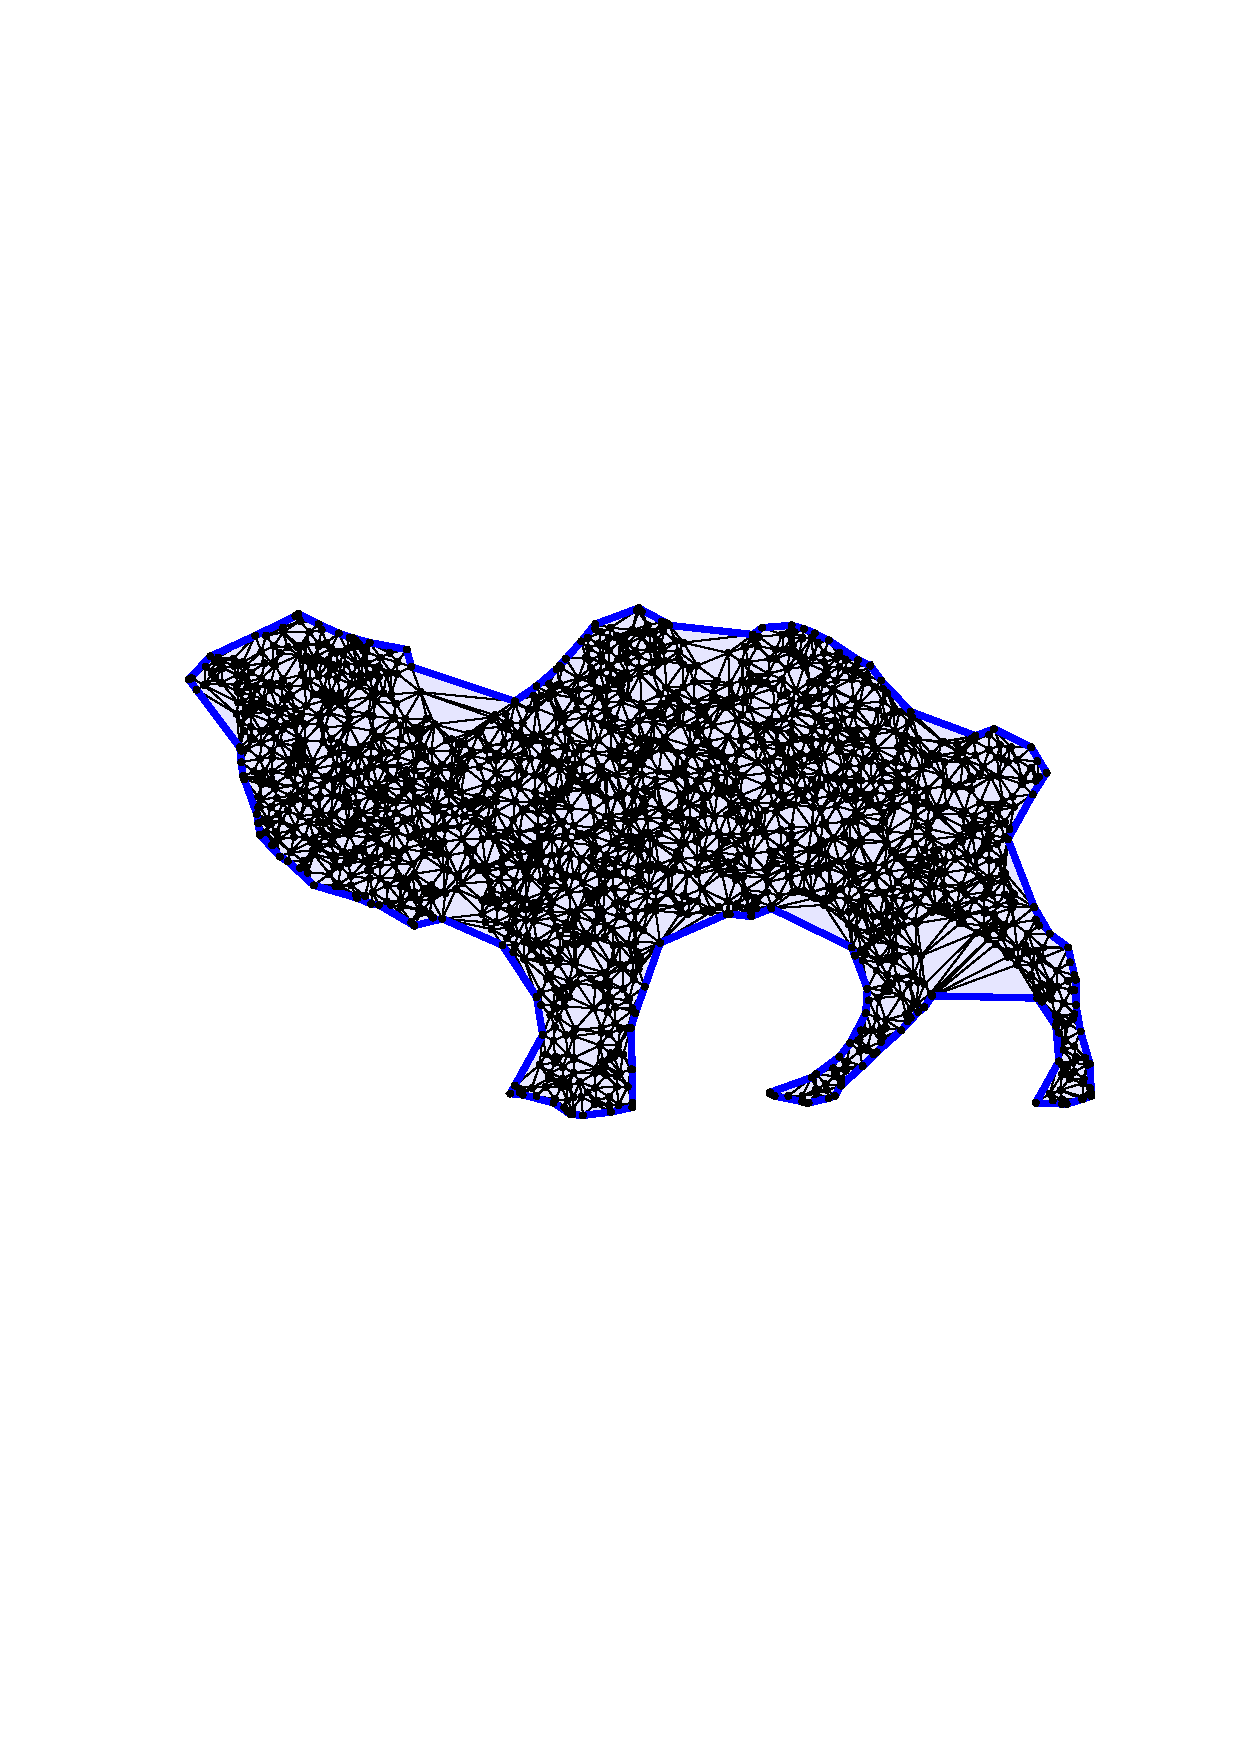
\includegraphics[width=4.25cm,height=3.75cm,trim={2.5cm 11cm 2.5cm 8cm},clip]{camel_alphashape_0.09.pdf}}}\hspace{.5cm}\\
\subfloat[$\alpha=0.1$]{{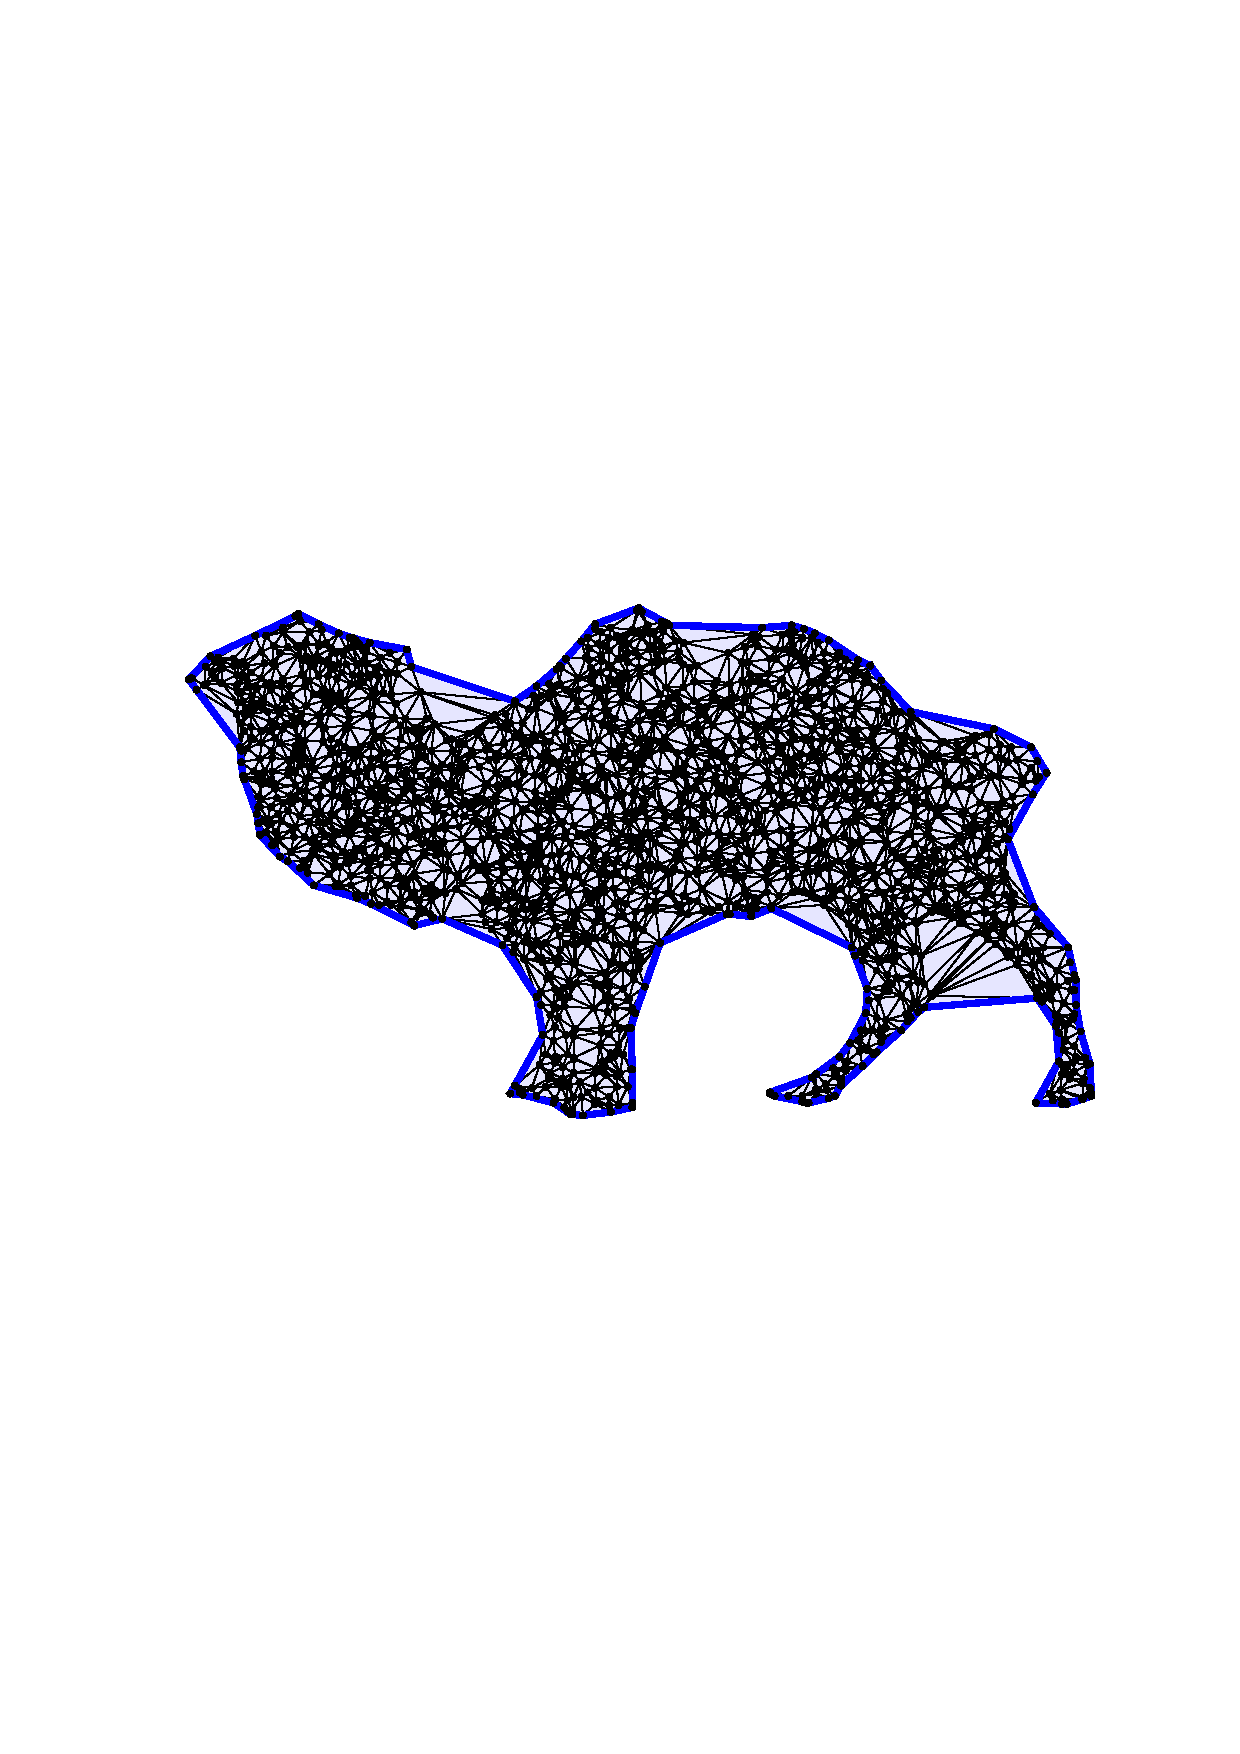
\includegraphics[width=4.25cm,height=3.75cm,trim={2.5cm 11cm 2.5cm 8cm},clip]{camel_alphashape_0.1.pdf}}}\hspace{.5cm}
\subfloat[$\alpha=0.3$]{{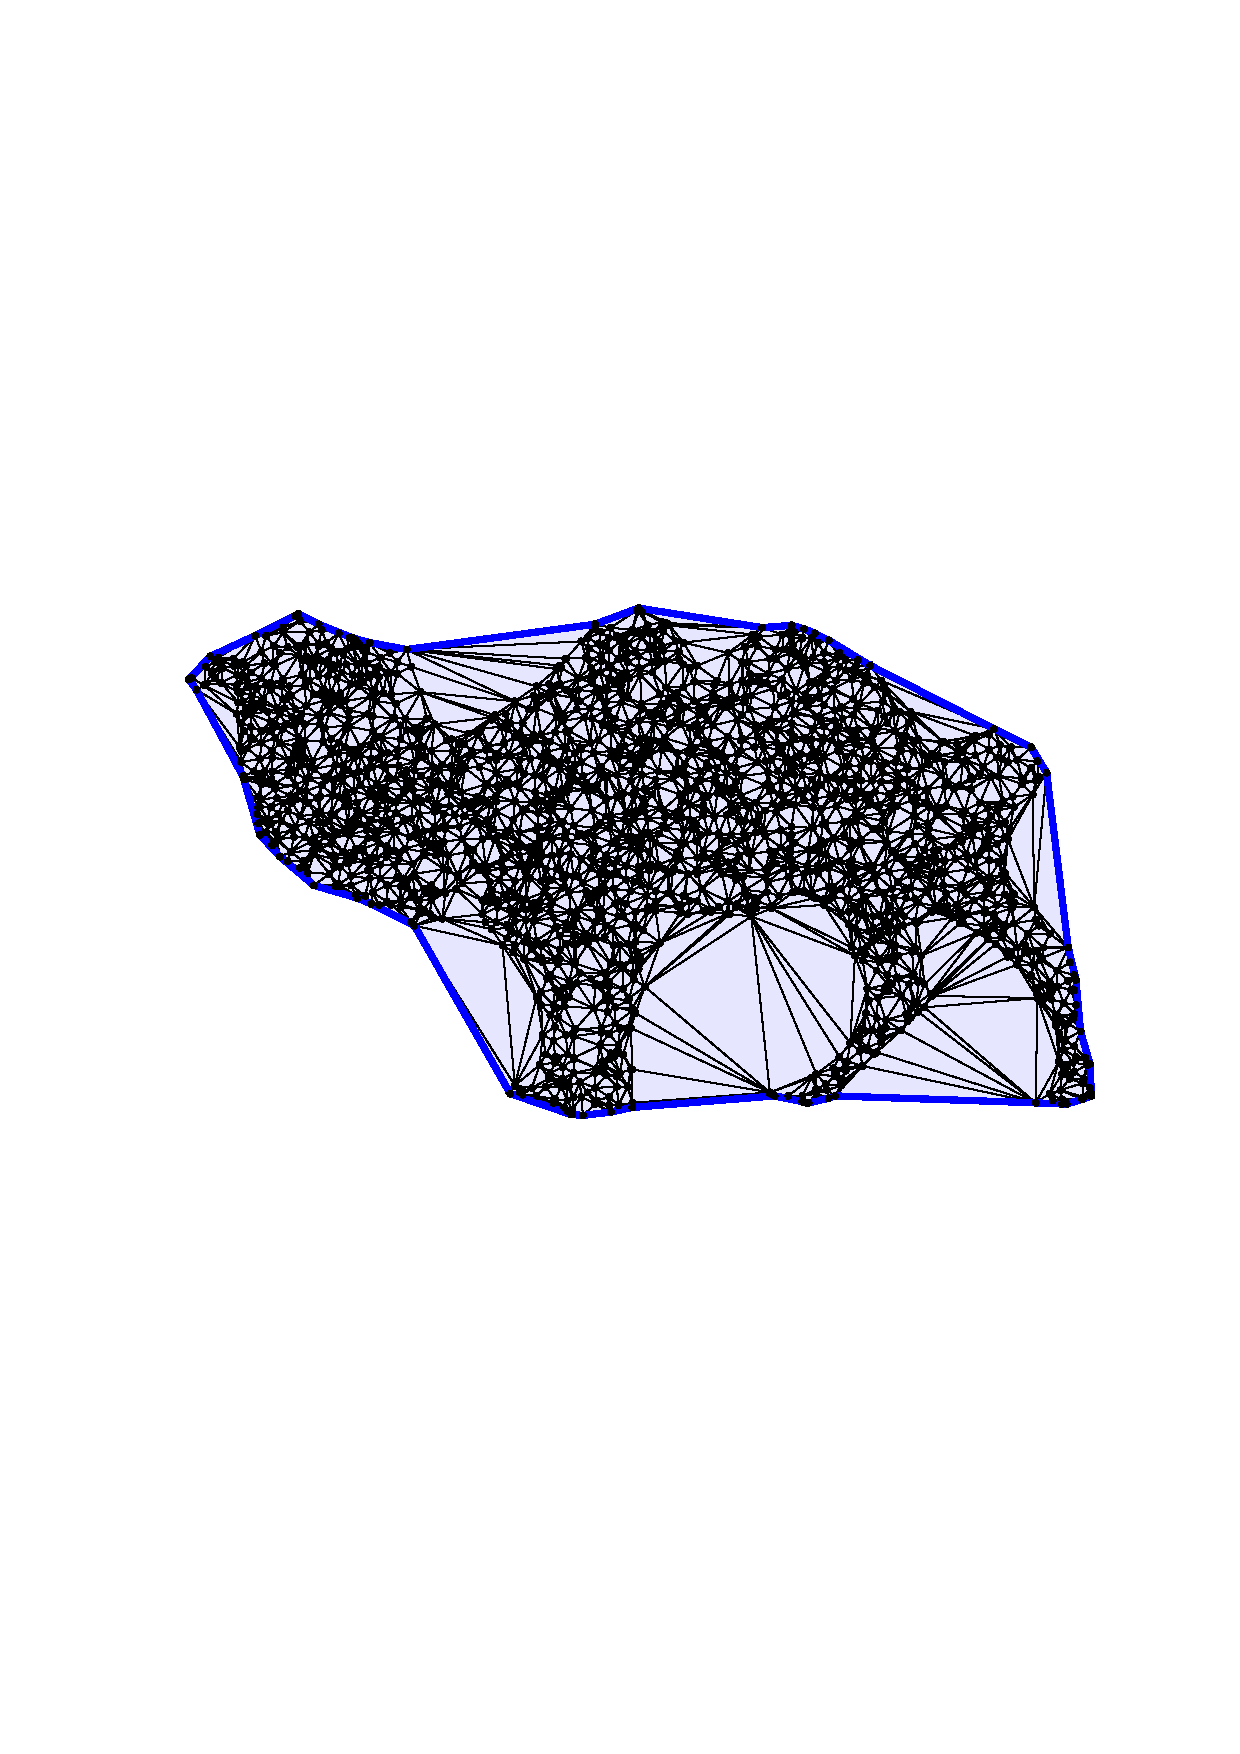
\includegraphics[width=4.25cm,height=3.75cm,trim={2.5cm 11cm 2.5cm 8cm},clip]{camel_alphashape_0.3.pdf}}}\hspace{.5cm}
\subfloat[$\alpha=0.9$]{{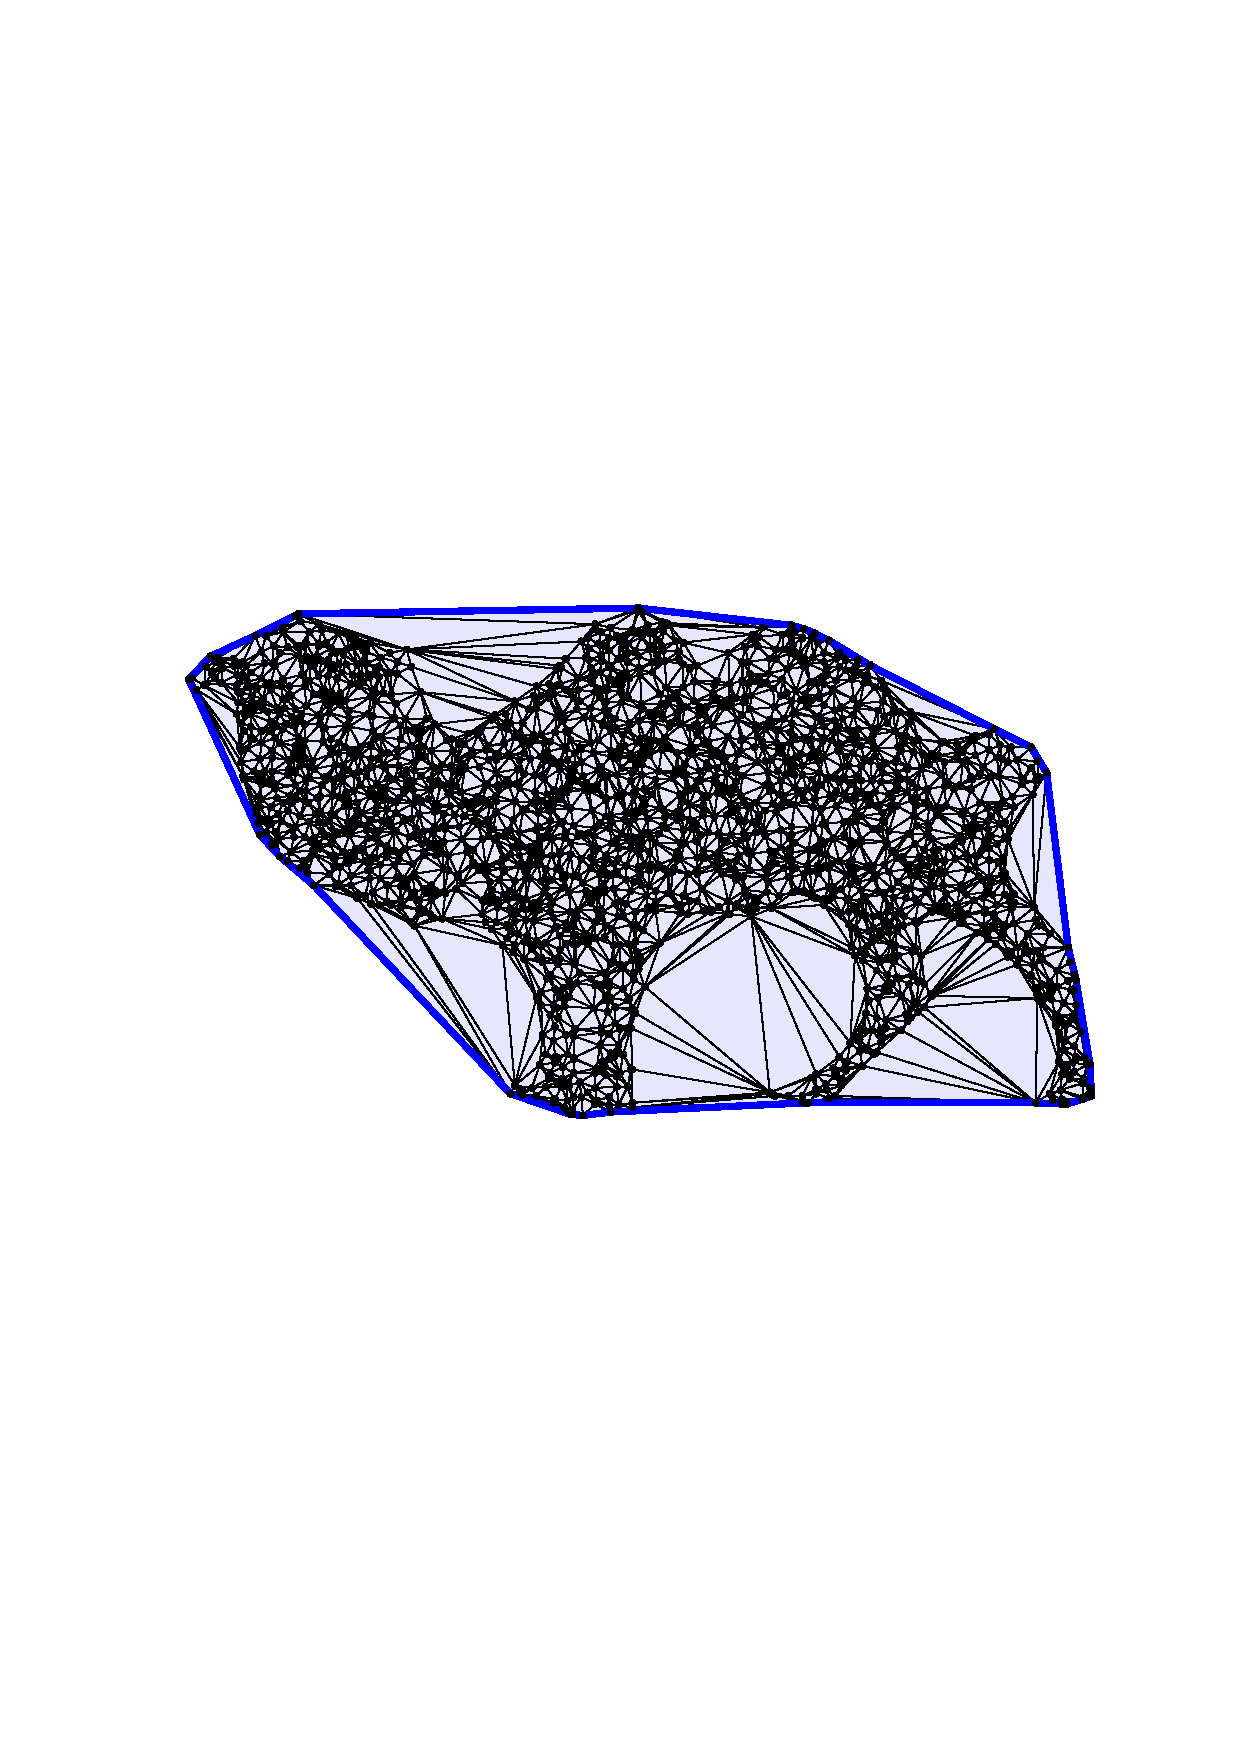
\includegraphics[width=4.25cm,height=3.75cm,trim={2.5cm 11cm 2.5cm 8cm},clip]{camel_alphashape_0.9.pdf}}}\hspace{.5cm}
\caption{Alpha-shapes for different values of $\alpha$.}
\label{fig:alphashapes:alphashapes}
\end{figure}

\begin{qbox}
\begin{enumerate}
\item Implement the algorithm : loop over all simplices of the Delaunay triangulation, and check if the radius is lower than $\alpha$. In this case, do not display this triangle.
\item Test this operator with the input data using different values of $\alpha$ (floating point parameter).
\end{enumerate}
\end{qbox}

\begin{pcomment}
The radius of the circumcircle is not difficult to compute, however, you may use the module \pinline{sympy} in order to compute it easily.

 \begin{python}
from sympy import Point, Triangle
p1, p2, p3 = Point(0, 0), Point(1, 0), Point(0, 1)
t = Triangle(p1, p2, p3)
print(t.circumradius)
 \end{python}

\end{pcomment}

